\documentclass[11pt]{article}
\usepackage[a4paper,margin=25mm,headheight=15pt]{geometry}
\usepackage[T1]{fontenc}
\usepackage[dvipsnames]{xcolor}
\usepackage{amsmath,amsthm,booktabs,array,mathtools}
\usepackage{newtxtext,newtxmath}
\usepackage{microtype}
\usepackage{tikz}
\usepackage[most]{tcolorbox}
\usepackage{enumitem,fancyhdr,lastpage}
\usepackage{listings}
\usepackage[colorlinks=true,linkcolor=MidnightBlue,citecolor=MidnightBlue,urlcolor=TealBlue]{hyperref}
\definecolor{ink}{HTML}{19344B}
\definecolor{accent}{HTML}{137C83}
\definecolor{pale}{HTML}{EFF6F7}
\hypersetup{pdftitle={A bicyclic 30-vertex graph with domination root -4},
 pdfauthor={Research note prepared with ChatGPT},
 pdfsubject={Exact counterexample to 33-vertex minimality; reproducible certificates}}
\pagestyle{fancy}
\fancyhf{}
\fancyhead[L]{\small\sffamily\color{ink}A 30-vertex domination-root certificate}
\fancyhead[R]{\small\sffamily Research note}
\fancyfoot[L]{\small\sffamily 18 September 2026}
\fancyfoot[R]{\small\sffamily\thepage\ / \pageref*{LastPage}}
\renewcommand{\headrulewidth}{0.3pt}
\setlength{\parindent}{0pt}
\setlength{\parskip}{5.5pt plus 1pt minus 1pt}
\setlength{\emergencystretch}{2em}
\numberwithin{equation}{section}
\newtheorem{theorem}{Theorem}[section]
\newtheorem{lemma}[theorem]{Lemma}
\newtheorem{proposition}[theorem]{Proposition}
\newtheorem{corollary}[theorem]{Corollary}
\theoremstyle{definition}
\newtheorem{definition}[theorem]{Definition}
\newtheorem{remark}[theorem]{Remark}
\newcommand{\D}{D}
\newcommand{\N}{N}
\newcommand{\Q}{\mathbb{Q}}
\newcommand{\Z}{\mathbb{Z}}
\newcommand{\Rtree}{\mathcal{R}}
\newcommand{\Gthirty}{G_{30}}
\newcommand{\supp}{\operatorname{supp}}
\newcommand{\tw}{\operatorname{tw}}
\newtcolorbox{resultbox}{colback=pale,colframe=accent,boxrule=0.7pt,
 arc=1mm,left=3mm,right=3mm,top=2mm,bottom=2mm}
\lstset{basicstyle=\small\ttfamily,breaklines=true,columns=fullflexible,
 frame=single,rulecolor=\color{accent},backgroundcolor=\color{pale},
 keepspaces=true,showstringspaces=false}
\begin{document}
\thispagestyle{empty}
{\sffamily\small\color{accent}\bfseries EXACT COMBINATORICS \quad / \quad RESEARCH CERTIFICATE}
\vspace{5mm}

{\LARGE\bfseries\color{ink}A bicyclic 30-vertex graph\par
with domination root \(\boldsymbol{-4}\)\par}
\vspace{3mm}
{\large A counterexample to the proposed 33-vertex minimum}

\vspace{2mm}
{\small Research note prepared with ChatGPT\hfill 18 September 2026}
\vspace{4mm}

\begin{abstract}
We construct a connected simple graph on 30 vertices and 31 edges whose
 domination polynomial has the simple integer root \(-4\). This answers
 negatively the explicit question whether 33 is the minimum possible order.
 The graph is planar, has treewidth two, and has domination number ten.
 The root certificate reduces to the rational identity
\[
21-\frac{5}{13}+\frac{256}{13}
 \left(-\frac12-\frac{35}{64}\right)=0.
\]
We prove the reduction, give the complete edge list and polynomial, and
 provide three mutually consistent exact polynomial certificates.
 A supported-edge construction gives connected planar examples at every
 order at least 32, and examples with arbitrarily high multiplicity at
 \(-4\). The accompanying dependency-free Python programs reproduce the
 discovery and verify the certificates. No claim is made that 30 is the
 true minimum order.
\end{abstract}

\begin{resultbox}
\textbf{Main exact result.}
There is a connected planar graph \(\Gthirty\) with
\[
 |V|=30,\qquad |E|=31,\qquad \tw(\Gthirty)=2,\qquad
 \D(\Gthirty,x)=x^{10}(x+4)Q_{19}(x),
\]
where \(Q_{19}\in\Z[x]\) and \(Q_{19}(-4)=-38\,318\,272\ne0\).
The graph, not merely an abstract existence argument, is specified below.
\end{resultbox}

\section{The question selected and the scope of the answer}

For a finite simple graph \(G=(V,E)\), a set \(S\subseteq V\) is
\emph{dominating} when every vertex outside \(S\) has a neighbor in \(S\).
The domination polynomial is the generating polynomial
\begin{equation}\label{eq:def}
 \D(G,x)=\sum_{\substack{S\subseteq V\\S\text{ dominating}}}x^{|S|}
        =\sum_{k=0}^{|V|}d(G,k)x^k.
\end{equation}
A domination root is a zero of this polynomial. The coefficients count
sets; all evaluations and cancellations in this note are exact.

Alikhani and Griswold \cite{AG} gave a 33-vertex graph with domination
root \(-4\), already disproving the earlier conjecture that the only
integer domination roots are \(0\) and \(-2\). Their Section~4, question~2,
asks whether 33 is minimal. We attack that follow-up question, not the
already-refuted original conjecture. The present construction shows that
33 is \emph{not} minimal. It also reduces the cyclomatic number from four
in their example to two.

The result is an explicit finite certificate with a conventional proof.
It is not a claim of a globally smallest graph, a classification of
integer domination roots, or a resolution of whether \(-6\) occurs.
Literature searches through the date of this note did not locate the
same improvement, but cannot establish publication priority. Independent
human review remains appropriate before making a novelty claim in a
submission.

\section{The graph and its elementary invariants}\label{sec:graph}

Let \(V(\Gthirty)=\{0,1,\ldots,29\}\). Its edge set is the following
set of unordered pairs:
\begin{equation}\label{eq:edges}
\begin{aligned}
E(\Gthirty)=\{&
\{0,1\},\{1,2\},\{2,3\},\{3,0\},\{1,4\},\{2,4\},\\
&\{4,5\},\{4,6\},\{4,7\},\{4,8\},\{4,9\},\{1,10\},\{10,11\},\\
&\{2,12\},\{12,13\},\{12,14\},\{14,15\},\{15,16\},\\
&\{14,17\},\{17,18\},\{14,19\},\{19,20\},\{14,21\},\\
&\{21,22\},\{21,23\},\{21,24\},\{3,25\},\{25,26\},\\
&\{25,27\},\{27,28\},\{28,29\}\}.
\end{aligned}
\end{equation}
For machine use, \texttt{data/graph30.json} and \texttt{data/edges.txt}
contain the same edge records as pairs of integers.

\begin{figure}[htbp]
\centering
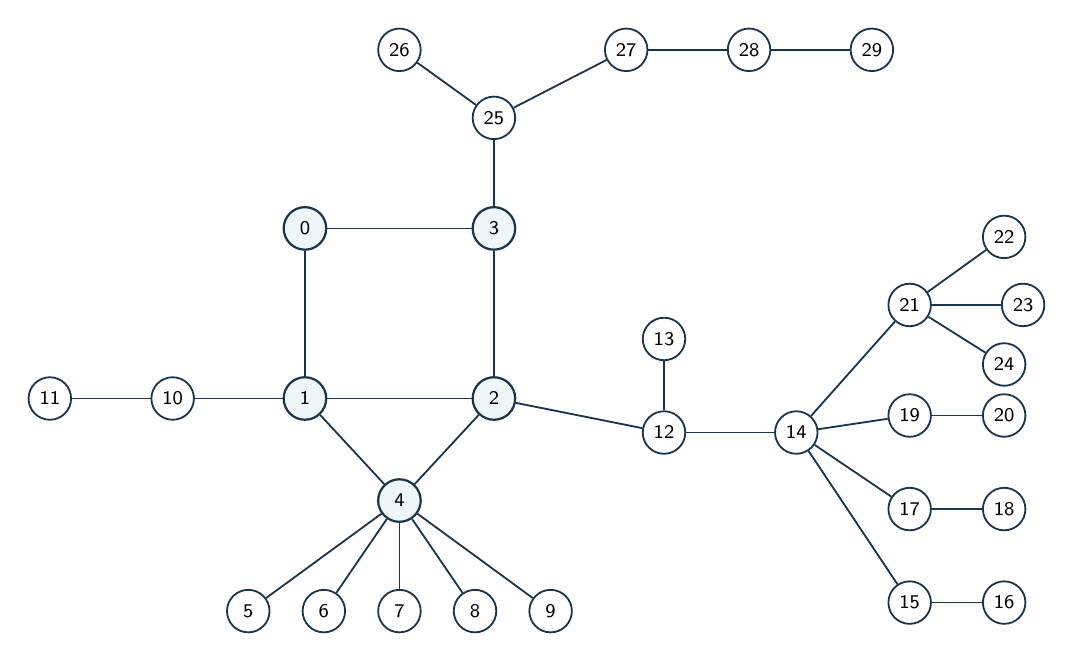
\begin{tikzpicture}[x=1.20cm,y=1.08cm,
 v/.style={circle,draw=ink,fill=white,inner sep=0pt,minimum size=5.4mm,
 font=\scriptsize\sffamily},
 core/.style={v,fill=pale,line width=0.8pt},
 every path/.style={draw=ink,line width=0.65pt}]
\node[core] (0) at (-1,2) {0};
\node[core] (1) at (-1,0) {1};
\node[core] (2) at (1,0) {2};
\node[core] (3) at (1,2) {3};
\node[core] (4) at (0,-1.2) {4};
\node[v] (5) at (-1.6,-2.5) {5};
\node[v] (6) at (-0.8,-2.5) {6};
\node[v] (7) at (0,-2.5) {7};
\node[v] (8) at (0.8,-2.5) {8};
\node[v] (9) at (1.6,-2.5) {9};
\node[v] (10) at (-2.4,0) {10};
\node[v] (11) at (-3.7,0) {11};
\node[v] (12) at (2.8,-0.4) {12};
\node[v] (13) at (2.8,0.7) {13};
\node[v] (14) at (4.2,-0.4) {14};
\node[v] (15) at (5.4,-2.4) {15};
\node[v] (16) at (6.4,-2.4) {16};
\node[v] (17) at (5.4,-1.3) {17};
\node[v] (18) at (6.4,-1.3) {18};
\node[v] (19) at (5.4,-0.2) {19};
\node[v] (20) at (6.4,-0.2) {20};
\node[v] (21) at (5.4,1.1) {21};
\node[v] (22) at (6.4,1.9) {22};
\node[v] (23) at (6.6,1.1) {23};
\node[v] (24) at (6.4,0.4) {24};
\node[v] (25) at (1,3.3) {25};
\node[v] (26) at (0,4.1) {26};
\node[v] (27) at (2.4,4.1) {27};
\node[v] (28) at (3.7,4.1) {28};
\node[v] (29) at (5,4.1) {29};
\foreach \u/\v in {0/1,1/2,2/3,3/0,1/4,2/4,
4/5,4/6,4/7,4/8,4/9,1/10,10/11,2/12,12/13,12/14,
14/15,15/16,14/17,17/18,14/19,19/20,14/21,21/22,21/23,21/24,
3/25,25/26,25/27,27/28,28/29}{\draw (\u)--(\v);}
\end{tikzpicture}
\caption{The exact 30-vertex graph. Shaded vertices form its five-vertex
2-core. The displayed drawing is planar.}
\label{fig:graph}
\end{figure}

An equivalent structural description starts with the cycle
\(0-1-2-3-0\). Add a common neighbor \(4\) of vertices \(1,2\), and give
\(4\) five leaves. Attach to vertex \(1\) a two-vertex rooted path.
Attach to vertex \(2\) the rooted tree on vertices \(12,\ldots,24\).
Attach to vertex \(3\) the rooted tree on vertices \(25,\ldots,29\).
Only the root of each attached tree meets the cycle, by one added edge.
Vertex \(0\) has no attached tree.

\begin{proposition}\label{prop:invariants}
The graph \(\Gthirty\) is connected and planar, has 30 vertices, 31 edges,
15 leaves, maximum degree seven, cyclomatic number two, treewidth two,
and domination number ten.
\end{proposition}
\begin{proof}
The construction gives connectivity and the counts directly. Removing
all pendant trees leaves the cycle together with the vertex \(4\) and
its two edges to \(1,2\). This core is planar; attaching trees preserves
planarity. For a connected graph the cyclomatic number is \(|E|-|V|+1\),
which here is \(31-30+1=2\).

For completeness, a tree decomposition of the core has the three bags
\[
 \{1,2,4\},\qquad \{0,1,2\},\qquad \{0,2,3\},
\]
joined in the displayed order. Every core edge lies in a bag, and the
bags containing any fixed vertex form a connected subtree. Attach one
bag \(\{u,v\}\) for each edge in a pendant tree, extending from the bag
containing its parent vertex. The largest bag has size three, so the
width is at most two. The graph contains a cycle and is not a forest,
so its treewidth is not at most one.

To establish the domination number without the polynomial calculation,
consider the nine pairwise disjoint closed neighborhoods of leaves
\[
 \{4,5\},\{10,11\},\{12,13\},\{15,16\},\{17,18\},
 \{19,20\},\{21,22\},\{25,26\},\{28,29\}.
\]
Every dominating set must meet each one. It must also meet
\(N[0]=\{0,1,3\}\), disjoint from all nine. Thus its size is at least ten.
The set
\[
 \{0,4,10,12,15,17,19,21,25,28\}
\]
dominates every vertex, proving the matching upper bound.
\end{proof}

The cyclomatic number has an additional interpretation. Oboudi's
Theorem~7 \cite{Oboudi} excludes integer roots other than \(0,-2\) for
trees and unicyclic graphs. Combining that published result with the
construction below gives
\begin{equation}\label{eq:mincycle}
\min\{|E(G)|-|V(G)|+1:\ G\text{ connected},\ \D(G,-4)=0\}=2.
\end{equation}
The upper bound in \eqref{eq:mincycle} is proved here; its lower bound
uses the cited theorem. This is an exact minimum of \emph{cycle rank},
not an assertion that 30 is a minimum of \emph{order}.

\section{Rooted-tree states: the local calculation}\label{sec:states}

The three-state recurrence below is elementary. We include the details
so that the root certificate does not rely on any black-box graph
polynomial implementation.

\begin{definition}
For a tree \(T\) with distinguished root \(v\), let \(A_T,B_T,C_T\in\Z[x]\)
be the weighted sums of subsets of \(V(T)\) with these respective
properties:
\begin{enumerate}[label=(\alph*),leftmargin=7mm,itemsep=1pt,topsep=2pt]
\item every vertex is dominated and \(v\) is selected;
\item every vertex is dominated and \(v\) is not selected;
\item every vertex except \(v\) is dominated, and \(v\) is not dominated.
\end{enumerate}
The weight of a subset \(S\) is \(x^{|S|}\). In state \(C_T\), the root
is necessarily unselected. Set \(P_T=A_T+B_T=\D(T,x)\).
\end{definition}

Write \(\Rtree(T_1,\ldots,T_s)\) for the rooted tree obtained by adjoining
one new root and joining it to the roots of disjoint copies of
\(T_1,\ldots,T_s\). In particular, \(L=\Rtree()\) is one vertex.

\begin{lemma}[Rooted recurrence]\label{lem:recurrence}
For \(T=\Rtree(T_1,\ldots,T_s)\),
\begin{align}
 A_T&=x\prod_{j=1}^s(A_{T_j}+B_{T_j}+C_{T_j}),\label{eq:A}\\
 B_T&=\prod_{j=1}^s(A_{T_j}+B_{T_j})-\prod_{j=1}^sB_{T_j},\label{eq:B}\\
 C_T&=\prod_{j=1}^sB_{T_j}.\label{eq:C}
\end{align}
Empty products are one, so \((A_L,B_L,C_L)=(x,0,1)\).
\end{lemma}
\begin{proof}
If the new root is selected, it contributes \(x\), and each child root
may be in any of the three states: a formerly undominated child root
is now dominated by its selected parent. This proves \eqref{eq:A}.
If the new root is unselected, each child subtree must internally
dominate its own root, allowing only \(A\) and \(B\). Among these
choices, precisely those in which every child is in state \(B\) leave
the new root undominated. Subtracting that class gives \eqref{eq:B},
and retaining it gives \eqref{eq:C}. All decompositions preserve the
number of selected vertices, proving the polynomial identities.
\end{proof}

If a rooted tree has a leaf immediately adjacent to its root, then
\(C_T=0\) as a polynomial: such a leaf contributes the factor \(B_L=0\)
to \eqref{eq:C}. Combinatorially, an undominated root would force its
private leaf to be both unselected and undominated.

For our graph define
\begin{align*}
 E&=\Rtree(L), &J&=\Rtree(E), &S_3&=\Rtree(L,L,L),\\
 W&=\Rtree(E,E,E,S_3), &T&=\Rtree(L,W), &K&=\Rtree(L,J),\\
 S_5&=\Rtree(L,L,L,L,L).&&&&
\end{align*}
The four external gadgets are \(E,T,K,S_5\), of orders \(2,13,5,6\).
Their roots are respectively the vertices \(10,12,25,4\). The first
three attach to one cycle vertex; the last attaches to both \(1,2\).
Each of the four has \(C=0\) identically.

\begin{table}[htbp]
\centering
\small
\begin{tabular}{lrrrrr}
\toprule
Tree & Order & \(A(-4)\) & \(B(-4)\) & \(C(-4)\) & \(B/(A+B)\) at \(-4\)\\
\midrule
\(L\)   &1&\(-4\)&0&1& ---\\
\(E\)   &2&12&\(-4\)&0&\(-1/2\)\\
\(J\)   &3&\(-32\)&12&\(-4\)& ---\\
\(S_3\) &4&108&\(-64\)&0&\(-16/11\)\\
\(W\)   &11&\(-90\,112\)&\(18\,432\)&\(4\,096\)& ---\\
\(T\)   &13&\(-811\,008\)&\(286\,720\)&0&\(-35/64\)\\
\(K\)   &5&\(-288\)&80&0&\(-5/13\)\\
\(S_5\) &6&972&\(-1\,024\)&0&\(256/13\)\\
\bottomrule
\end{tabular}
\caption{Exact rooted states. Dashes suppress ratios not used as
zero-\(C\) attachments. Every entry follows from
Lemma~\ref{lem:recurrence}.}
\label{tab:states}
\end{table}

Here are the larger arithmetic steps, to make the table checkable by
hand. For \(E\), \(A+B=8\); for \(S_3\), \(A+B=44\). Thus
\begin{align*}
 A_W&=-4\cdot8^3\cdot44=-90\,112,\\
 B_W&=8^3\cdot44-(-4)^3(-64)=18\,432,\qquad C_W=4\,096.
\end{align*}
Therefore \(A_W+B_W+C_W=-67\,584\), while
\(A_W+B_W=-71\,680\). Adding the new root and its leaf gives
\begin{align*}
 A_T&=-4(-3)(-67\,584)=-811\,008,\\
 B_T&=(-4)(-71\,680)=286\,720,\qquad C_T=0.
\end{align*}
Likewise \((A_J,B_J,C_J)=(-32,12,-4)\), and hence
\(A_K=-4(-3)(-24)=-288\), \(B_K=(-4)(-20)=80\).
Finally \(A_{S_5}=-4(-3)^5=972\) and \(B_{S_5}=(-4)^5=-1024\).

\section{A four-cycle identity and the root proof}\label{sec:identity}

We now prove the identity that turns the table into a root certificate.
Although the search used weighted states at one value of \(x\), all four
gadgets in the final graph satisfy the stronger polynomial condition
\(C=0\).

\begin{proposition}[One hub and one undecorated corner]\label{prop:cycle}
Start with \(C_4\) on \(0,1,2,3\). Attach zero-\(C\) rooted gadgets
\(F_1,F_2,F_3\) to vertices \(1,2,3\), respectively, and attach a
zero-\(C\) rooted gadget \(H\) by joining its root to both \(1,2\).
No gadget is attached to \(0\). Write
\[
 P_i=A_i+B_i,\quad P_H=A_H+B_H,\quad
 a=\frac{B_1}{P_1},\quad b=\frac{B_2}{P_2},\quad
 c=\frac{B_3}{P_3},\quad r=\frac{B_H}{P_H},\quad
 \mathcal P=P_1P_2P_3P_H.
\]
As an identity of rational functions (and after clearing denominators,
of polynomials), the resulting graph \(G\) satisfies
\begin{equation}\label{eq:cycle}
 \D(G,x)=x\mathcal P\bigl[x^3+4x^2+6x+3-c-r(a+b)\bigr].
\end{equation}
\end{proposition}
\begin{proof}
First sum over configurations that dominate all gadget vertices but
impose no domination requirement on the four cycle vertices. A root
cannot be in state \(C\), so its total internal weight is \(P\),
independently of which adjacent cycle vertices are selected. The
unrestricted total is consequently \(\mathcal P(1+x)^4\).

Apply inclusion--exclusion to the events that specified cycle vertices
are undominated. For \(U\subseteq\{0,1,2,3\}\), this forces every cycle
vertex in \(N_{C_4}[U]\) to be unselected. The remaining cycle vertices
contribute \((1+x)^{4-|N_{C_4}[U]|}\). Every attached root meeting a
vertex of \(U\) must also be unselected, replacing its factor \(P\) by
\(B\). In particular, the shared root contributes \(r\) once whenever
\(U\cap\{1,2\}\ne\varnothing\), not twice. With
\(u_0=1,u_1=a,u_2=b,u_3=c\), this gives
\begin{equation}\label{eq:IE}
 \frac{\D(G,x)}{\mathcal P}=
 \sum_{U\subseteq\{0,1,2,3\}}
 (-1)^{|U|}(1+x)^{4-|N_{C_4}[U]|}
 \prod_{i\in U}u_i\,
 r^{\mathbf1_{U\cap\{1,2\}\ne\varnothing}}.
\end{equation}

Put \(t=1+x\). The empty-set contribution is \(t^4\), and singleton
contributions sum to \(-t[1+c+r(a+b)]\). Any two distinct cycle
vertices have closed-neighborhood union equal to the entire cycle.
The contributions by cardinality two, three and four are therefore
\begin{align*}
 &c+r(a+b+ab+ac+bc),\\
 &-r(ab+ac+bc+abc),\\
 &rabc,
\end{align*}
whose sum is \(c+r(a+b)\). Thus \eqref{eq:IE} becomes
\[
 t^4-t+(1-t)[c+r(a+b)]
 =x[x^3+4x^2+6x+3-c-r(a+b)],
\]
proving the assertion. Clearing denominators also proves the identity
at values where a displayed ratio is undefined.
\end{proof}

\begin{theorem}[The counterexample]\label{thm:root}
The graph specified by \eqref{eq:edges} satisfies \(\D(\Gthirty,-4)=0\).
Consequently, the answer to the 33-vertex minimality question is no.
\end{theorem}
\begin{proof}
Apply Proposition~\ref{prop:cycle} with
\(F_1=E,F_2=T,F_3=K,H=S_5\). At \(x=-4\),
\[
 (P_1,P_2,P_3,P_H)=(8,-524\,288,-208,-52),
 \qquad \mathcal P=-45\,365\,592\,064\ne0.
\]
Table~\ref{tab:states} gives
\[
 a=-\frac12,\qquad b=-\frac{35}{64},\qquad
 c=-\frac5{13},\qquad r=\frac{256}{13}.
\]
At \(-4\), the bracket in \eqref{eq:cycle} is
\(-21-c-r(a+b)\). But
\[
 a+b=-\frac{67}{64},\qquad r(a+b)=-\frac{268}{13},
 \qquad 21+c=\frac{268}{13}.
\]
The bracket is exactly zero. Equivalently,
\begin{equation}\label{eq:oneline}
 \frac{\D(\Gthirty,-4)}{4\mathcal P}
 =21-\frac5{13}+\frac{256}{13}
   \left(-\frac12-\frac{35}{64}\right)=0.
\end{equation}
This is an equality in \(\Q\), not a numerical approximation.
\end{proof}

\begin{remark}
The proof uses only the explicit graph and the elementary state and
inclusion--exclusion identities proved above. It does not assume the
correctness of a numerical factorization, any search program, or any
particular normalization of the transfer matrices in earlier work.
\end{remark}

\section{The full polynomial and independent certificates}\label{sec:polynomial}

The nonzero coefficients are listed in Table~\ref{tab:coeff}.
All coefficients below degree ten vanish. The last coefficient is one,
as required because the whole vertex set is the unique set of size 30.

\begin{table}[htbp]
\centering
\begin{tabular}{rrrrrr}
\toprule
\(k\)&\(d(G,k)\)&\(k\)&\(d(G,k)\)&\(k\)&\(d(G,k)\)\\
\midrule
10&256&17&4\,526\,996&24&342\,684\\
11&4\,192&18&5\,803\,019&25&99\,255\\
12&32\,576&19&6\,049\,225&26&22\,114\\
13&159\,418&20&5\,150\,665&27&3\,651\\
14&550\,047&21&3\,583\,938&28&420\\
15&1\,420\,449&22&2\,031\,824&29&30\\
16&2\,845\,950&23&932\,405&30&1\\
\bottomrule
\end{tabular}
\caption{The complete nonzero coefficient list of \(\D(\Gthirty,x)\).}
\label{tab:coeff}
\end{table}

Exact division gives
\begin{equation}\label{eq:factor}
 \D(\Gthirty,x)=x^{10}(x+4)Q_{19}(x),
\end{equation}
where
\begin{equation}\label{eq:quotient}
\begin{aligned}
Q_{19}(x)={}&x^{19}+26x^{18}+316x^{17}+2387x^{16}+12566x^{15}\\
 &+48991x^{14}+146720x^{13}+345525x^{12}+649724x^{11}\\
 &+985042x^{10}+1210497x^9+1207237x^8+974071x^7\\
 &+630712x^6+323102x^5+128041x^4+37883x^3\\
 &+7886x^2+1032x+64.
\end{aligned}
\end{equation}
No irreducibility assertion is needed. Substitution yields
\begin{equation}\label{eq:simple}
 Q_{19}(-4)=-38\,318\,272,\qquad
 \D'(\Gthirty,-4)=(-4)^{10}Q_{19}(-4)
 =-40\,179\,620\,380\,672\ne0.
\end{equation}
This proves that \(-4\) is a simple root.

\subsection{Certificate A: expansion of the four-cycle identity}

Proposition~\ref{prop:cycle} has the denominator-free form
\begin{equation}\label{eq:denfree}
\begin{aligned}
\D(G,x)=x\bigl[&
 (x^3+4x^2+6x+3)P_1P_2P_3P_H\\
 &-B_HP_3(B_1P_2+B_2P_1)-B_3P_1P_2P_H\bigr].
\end{aligned}
\end{equation}
The following compact gadget polynomials, together with
\eqref{eq:denfree}, are one symbolic certificate for every coefficient.
Let
\[
 p=x(x+2),\qquad s=x(1+x)^3+x^3.
\]
Then
\begin{align}
 P_1&=p,& B_1&=x,\notag\\
 P_H&=x(1+x)^5+x^5,&B_H&=x^5,\notag\\
 P_3&=x^2(x^3+5x^2+8x+3),&B_3&=x^2(x^2+3x+1),\label{eq:gadgetpolys}\\
 P_2&=x(x+1)(x+2)p^3s-x^7,&
 B_2&=x(x+1)p^3s-x^7.\notag
\end{align}
These follow directly from Lemma~\ref{lem:recurrence}. Expanding
\eqref{eq:denfree} with \eqref{eq:gadgetpolys} gives
Table~\ref{tab:coeff} and \eqref{eq:factor}.

\subsection{Certificate B: stripping trees and enumerating the 2-core}

Remove vertices of current degree zero or one successively. At a
removed vertex, compute its three rooted polynomial states and absorb
them into its surviving neighbor. The remaining 2-core here has five
vertices: \(0,1,2,3,4\).

At each remaining core vertex \(v\), let
\[
 T_v=\prod_j(A_j+B_j+C_j),\qquad
 U_v=\prod_j(A_j+B_j),\qquad V_v=\prod_j B_j,
\]
where the product runs over its absorbed child trees. For a selected
core subset \(S\), the local contribution of \(v\) is
\begin{equation}\label{eq:coreDP}
 \begin{cases}
 xT_v,&v\in S,\\
 U_v,&v\notin S\text{ and }N_{\rm core}(v)\cap S\ne\varnothing,\\
 U_v-V_v,&v\notin S\text{ and }N_{\rm core}(v)\cap S=\varnothing.
 \end{cases}
\end{equation}
Multiplying local factors and summing over all \(2^5=32\) subsets gives
the full polynomial. Formula~\eqref{eq:coreDP} is exactly the distinction
between root selected, root dominated by a core neighbor, and root
needing domination from a child. Thus it counts each dominating set
once. This calculation does not use the special four-cycle identity.

\subsection{Certificate C: an independent enumeration over non-leaves}

The following identity avoids rooted states and 2-core stripping
altogether.

\begin{proposition}[Leaf-subset certificate]\label{prop:leaf}
Let \(G\) be a finite graph with no component isomorphic to \(K_2\).
Let \(L\) be its set of degree-one vertices and \(C=V\setminus L\).
For \(v\in C\), set \(t_v=|N(v)\cap L|\). Call \(S\subseteq C\)
admissible when every \(v\in C\) with \(t_v=0\) is dominated by \(S\)
in \(G[C]\). Then
\begin{equation}\label{eq:leaf}
 \D(G,x)=\sum_{S\text{ admissible}}
 x^{\,|S|+\sum_{v\in C\setminus S}t_v}
 (1+x)^{\sum_{v\in S}t_v}.
\end{equation}
\end{proposition}
\begin{proof}
Fix the selected non-leaves \(S\). If a non-leaf \(v\) is selected,
its adjacent leaves may each be selected or not, independently, giving
\((1+x)^{t_v}\). If \(v\) is not selected, every one of those leaves
must be selected, contributing \(x^{t_v}\). When \(t_v>0\), these
forced leaves also dominate \(v\). When \(t_v=0\), the only way to
dominate an unselected \(v\) is through the selected non-leaves; this
is precisely admissibility. The exclusion of isolated-edge components
ensures that every leaf has a non-leaf neighbor. These disjoint cases
exhaust all dominating sets and prove \eqref{eq:leaf}.
\end{proof}

For \(\Gthirty\), \(|L|=|C|=15\), so the independent computation tests
\(2^{15}=32768\) non-leaf subsets. Exactly 23065 are admissible.
Grouping the summands in \eqref{eq:leaf} by their two exponents gives
118 terms \(m_{a,b}x^a(1+x)^b\). The file
\texttt{data/leaf\_certificate.csv} records all triples \((a,b,m_{a,b})\).
Binomial expansion reproduces Table~\ref{tab:coeff}, and direct
substitution in that 118-term sum gives zero at \(-4\).

\section{Connected families and arbitrary multiplicity}\label{sec:families}

There is a simple way to preserve the root without leaving connected
graphs. The underlying supported-edge factorization is elementary and
related to the pendant-star products in Oboudi \cite{Oboudi}; it is not
claimed as a new general principle here.

Call a vertex a \emph{support vertex} when it has a neighbor of degree
one, called a private leaf.

\begin{lemma}[Edges between support vertices]\label{lem:support}
Suppose distinct vertices \(u,v\) each have a private leaf outside
\(\{u,v\}\), and these leaves remain private after the edge \(uv\) is
added or deleted. Toggling \(uv\) does not change the
family of dominating vertex subsets, hence does not change the
domination polynomial.
\end{lemma}
\begin{proof}
A dominating set must select either a private leaf of \(u\) or \(u\)
itself, because it must dominate that leaf. Either choice already
dominates \(u\), independently of the edge \(uv\). The same holds for
\(v\). Every other vertex has exactly the same neighbors before and
after the change. Thus a vertex subset dominates one graph exactly
when it dominates the other.
\end{proof}

For disjoint graphs, independently choosing dominating sets proves
\begin{equation}\label{eq:product}
 \D(G\mathbin{\dot\cup}H,x)=\D(G,x)\D(H,x).
\end{equation}
Combining this with the lemma connects factors without changing the
product.

\begin{theorem}[A bounded-width connected family]\label{thm:family}
For each integer \(t\ge0\), there is a connected planar graph \(G_t\)
with \(30+2t\) vertices, cyclomatic number two, treewidth two, maximum
degree seven, and
\begin{equation}\label{eq:family}
 \D(G_t,x)=[x(x+2)]^t\D(\Gthirty,x).
\end{equation}
In particular, \(-4\) is a simple root of every \(\D(G_t,x)\).
\end{theorem}
\begin{proof}
For \(t=0\), use \(\Gthirty\). For \(t\ge1\), take \(\Gthirty\) and
\(t\) disjoint edges \(a_i b_i\). Retain each
\(b_i\) as a private leaf. Join vertex \(10\) to \(a_1\), and join
\(a_i\) to \(a_{i+1}\) for \(1\le i<t\). Vertex \(10\) retains its
leaf \(11\). Each added connecting edge joins support vertices and
therefore changes no dominating sets. Since
\(\D(K_2,x)=2x+x^2=x(x+2)\), equations
\eqref{eq:product} and \eqref{eq:family} follow.

The new part is a pendant tree, so planarity, treewidth two, and cycle
rank two are preserved. There are \(2t\) new vertices and \(2t\) new
edges. Vertex \(10\) acquires at most one new incident edge; every
\(a_i\) has degree at most three. The old degree-seven vertex \(4\)
remains, so the maximum degree is still seven. Finally
\((-4)(-4+2)=8\ne0\), so multiplication by \([x(x+2)]^t\) does not
alter the multiplicity at \(-4\).
\end{proof}

\begin{corollary}[All sufficiently large orders]\label{cor:orders}
There is a connected planar graph of treewidth two and cycle rank two
with domination root \(-4\) at order 30 and at every order \(n\ge32\).
\end{corollary}
\begin{proof}
Besides attaching an isolated edge as above, we may attach a disjoint
star \(K_{1,2}\) by its center to a support vertex. Lemma~\ref{lem:support}
gives an additional factor
\[
 \D(K_{1,2},x)=x(1+x)^2+x^2=x(x^2+3x+1).
\]
At \(-4\) this factor is \(-20\ne0\); it adds three vertices and a
pendant tree. Every integer \(n-30\ge2\) is a nonnegative integer
combination of two and three. Using one three-vertex attachment for
odd \(n-30\), and otherwise only two-vertex attachments, proves the
claim. This construction asserts nothing about order 31.
\end{proof}

\begin{theorem}[Unbounded root multiplicity in connected graphs]\label{thm:mult}
For every integer \(k\ge1\), there is a connected planar graph \(H_k\)
of order \(30k\), treewidth two, and maximum degree seven in which
\(-4\) has multiplicity exactly \(k\).
\end{theorem}
\begin{proof}
Take \(k\) disjoint copies of \(\Gthirty\), and connect their copies
of vertex \(10\) in a path. Every connecting edge joins support
vertices retaining private leaves. Thus
\[
 \D(H_k,x)=\D(\Gthirty,x)^k.
\]
The root has multiplicity exactly \(k\) by \eqref{eq:simple}. The
connecting edges are bridges, so they preserve planarity and do not
increase treewidth beyond two. Internal copies of vertex \(10\) have
degree four after the operation; the maximum degree is still seven.
\end{proof}

These results strengthen the bare infinite-family question in
\cite[Section~4, question~3]{AG}: disconnected examples would follow
immediately from disjoint union, whereas the constructions here remain
connected and structurally sparse.

\section{How the search was made finite and reproducible}\label{sec:search}

The successful search was not a uniform enumeration of 30-vertex
graphs. It used the sparse core to turn a combinatorial search into
rational arithmetic on a catalogue of small rooted trees.

\subsection{The catalogue and the exact target equation}

A rooted tree is stored as the canonically ordered tuple of the shapes
of its children. The empty tuple is a leaf. Recursively enumerate
multisets of previously generated trees whose total order is \(n-1\),
then place a new root above them. This generates each unlabeled rooted
tree of order \(n\) exactly once: deleting the root yields a uniquely
determined multiset of rooted child components.

For each tree compute \((A(-4),B(-4),C(-4))\) by
Lemma~\ref{lem:recurrence}. Retain its rational ratio
\[
 q=\frac{B(-4)}{A(-4)+B(-4)}
 \quad\text{when}\quad C(-4)=0,\quad A(-4)+B(-4)\ne0.
\]
The condition \(C(-4)=0\) is sufficient for a weighted search at the
single point \(-4\); it need not hold identically for every candidate.
All final gadgets happen to satisfy \(C(x)=0\) identically, which
makes the polynomial proof particularly clean.

At a cycle site, disjoint branches give a product of their ratios.
Store a least-order realization for every attainable product, including
the empty forest with ratio one and order zero. Discarding larger
realizations of the same ratio is valid for this search: they have
identical normalized effects at \(-4\), and cannot improve its order
objective. The catalogue contains all such minimum-cost products within
the prescribed forest-size budget.

For a shared star hub with \(m\ge1\) leaves,
\begin{equation}\label{eq:hubratio}
 r_m=\frac{(-4)^m}{-4(-3)^m+(-4)^m}
     =\frac{4^{m-1}}{4^{m-1}-3^m}.
\end{equation}
The denominator is nonzero, since a power of four cannot equal a
positive power of three. Leaving vertex \(0\) undecorated reduces the
root search, by Proposition~\ref{prop:cycle}, to
\begin{equation}\label{eq:searchtarget}
 c=-21-r_m(a+b).
\end{equation}
Thus enumerate two stored ratios \(a,b\), compute the required \(c\),
and look it up exactly. No tolerance or root approximation occurs.
If the three forests have sizes \(n_a,n_b,n_c\), the total order is
\begin{equation}\label{eq:cost}
 n=5+m+n_a+n_b+n_c.
\end{equation}
The hit has \((m,n_a,n_b,n_c)=(5,2,13,5)\), giving \(n=30\).

\subsection{The supplied run and its limitations}

The portable reconstruction program uses rooted trees and site forests
of order at most 14 and hub sizes \(1\le m\le15\). It starts with the
strict target \(n<33\), tries the five-leaf hub first, and then tests
the other permitted hub sizes. It retains improving hits and checks
the graph of every hit with the separate 2-core polynomial routine.
A representative completed run gives:
\begin{center}
\begin{tabular}{lr}
\toprule
Quantity & Recorded value\\
\midrule
Distinct single-tree ratios & 4\,198\\
Distinct forest ratios, including the empty forest & 6\,118\\
Exact rational candidate lookups & 2\,547\,880\\
Best order returned & 30\\
Time in the execution environment & 6.154 seconds\\
\bottomrule
\end{tabular}
\end{center}
The time is an observation on this environment, not a complexity bound
or a cross-machine promise. The deterministic counts and the hit are
stored in \texttt{results/search.json}. The number of rooted trees at
each order from 1 through 14 is also recorded there.

In this bounded search, no smaller realization was returned. That is
\emph{not} an exhaustive lower bound for all graphs, all bicyclic
graphs, or even all rooted attachments to this core: an individual
site forest was limited to 14 vertices. Searching other cores,
allowing a decorated fourth corner, or allowing larger individual
forests can escape the tested class. The abstract minimum remains open
in this note.

\subsection{Verification and computational trust}

The complete coefficient list was recomputed by all three routes in
Section~\ref{sec:polynomial}: the symbolic four-cycle certificate,
the 2-core state algorithm, and the independent leaf-subset identity.
The latter two are genuinely different enumerations, although all are
implemented in the same Python runtime. They are not independent
proof-assistant formalizations.

The two general graph algorithms were also compared against direct
enumeration of all vertex subsets for \emph{every labeled simple graph
on zero through five vertices}: 1100 graphs in total. Further checks
used 120 deterministically seeded graphs on six through nine vertices.
Five instances of the connected extension in Theorem~\ref{thm:family}
were checked as polynomial identities. All tests passed.

The verification run recorded about 0.23 seconds. The important
properties are the exact outputs, not the timing. All polynomial
arithmetic is integer arithmetic, and all search ratios use Python's
\texttt{fractions.Fraction}. No symbolic algebra package, network
service, cached pickle, numerical optimizer, or proprietary system is
required to run the supplied code.

\section{Conclusions and remaining targets}\label{sec:conclusion}

The attack gives a concrete answer to the selected question: a graph
with domination root \(-4\) need not have 33 vertices. The explicit
order-30 example also demonstrates that cycle rank two and treewidth
two already suffice. The cancellation is additive in three rooted
ratios and a single shared-star ratio; it does not require a large
or highly connected core.

The demonstrated improvement is an \emph{upper bound}: the minimum
order is at most 30. A serious lower-bound project should canonicalize
possible small cores and carry exact rooted-state catalogues with a
global vertex budget, rather than infer minimality from an unsuccessful
restricted search. An especially natural next target is whether some
graph on at most 29 vertices has root \(-4\).

For other integer targets \(z\), the same core identity yields
\[
 c+r(a+b)=z^3+4z^2+6z+3,
\]
with the rooted states evaluated at \(z\). This provides a concrete
search equation, but this note establishes no graph with root \(-6\)
or \(-8\). Nor does it make a claim that all negative even integers
occur. The value of the present result is the fully specified,
independently checked counterexample and its complete elementary proof.

\appendix
\section{Reproducing the artifact}

The archive contains the \LaTeX{} source and compiled PDF, a
machine-readable edge list and coefficient table, the 118-term leaf
certificate, the exact verification report, and the reproducible
search program. From the archive's top directory, run
\begin{lstlisting}
python3 code/verify.py
python3 code/search.py
\end{lstlisting}
Python 3.10 or later is sufficient. The first command recomputes all
certificates, runs the tests, and writes
\texttt{results/verification.json}. The second reconstructs the rooted
catalogue from scratch and writes \texttt{results/search.json}.
Both commands stop with an error if their explicit verification checks
fail; the tests do not rely on Python's optionally disabled
\texttt{assert} statement.

To rebuild the document using a standard TeX Live installation:
\begin{lstlisting}
pdflatex -interaction=nonstopmode -halt-on-error domination_root_30.tex
pdflatex -interaction=nonstopmode -halt-on-error domination_root_30.tex
\end{lstlisting}
The graph drawing is embedded as TikZ code in this source. No external
image or font file is needed. The output PDF was rendered and visually
inspected before packaging.

\paragraph{Authorship and status.}
This note was produced in response to a request for an original
research attempt. The construction, proof, and verification artifacts
were developed in the session with ChatGPT. The note is not peer
reviewed and has not been formally verified in Lean. The exact finite
certificate is intended to make external checking straightforward.

\begin{thebibliography}{9}
\bibitem{AG}
S. Alikhani and M. Griswold,
\emph{On the Integer Domination Root Conjecture},
arXiv:2608.00109v1, 2026.
\href{https://arxiv.org/abs/2608.00109v1}{arxiv.org/abs/2608.00109v1}.
The selected minimality question is Section~4, question~2;
the infinite-family question is question~3. Accessed 18 September 2026.

\bibitem{Oboudi}
M. R. Oboudi,
\emph{On the roots of domination polynomial of graphs},
Discrete Applied Mathematics \textbf{205} (2016), 126--131.
\href{https://doi.org/10.1016/j.dam.2015.12.010}{doi:10.1016/j.dam.2015.12.010}.
Theorem~7 supplies the trees/unicyclic exclusion used in
\eqref{eq:mincycle}; Lemma~1 is the general domination
inclusion--exclusion identity.
\end{thebibliography}
\end{document}
